\documentclass{beamer}
\mode<presentation>
\usetheme{CambridgeUS}
\usepackage[russian]{babel}
\usepackage[utf8]{inputenc}
\usepackage[T2A]{fontenc}
\usepackage{sansmathaccent}

\usepackage{verbatim}
\usepackage{alltt}

\pdfmapfile{+sansmathaccent.map}
\title[Записи]{Комбинированный тип данных}
\author{Наумов Д.А., доц. каф. КТ, ИТГД }
\date[28.02.2020] {Программирование и алгоритмические языки, 2020}

\begin{document}

%ТИТУЛЬНЫЙ СЛАЙД
\begin{frame}
  \titlepage
\end{frame}
  
%СОДЕРЖАНИЕ ЛЕКЦИИ
\begin{frame}
  \frametitle{Содержание лекции}
  \tableofcontents  
\end{frame}
  
%РАЗДЕЛ 1
\section{Комбинированный тип данных}
\subsection{Описание комбинированного типа данных}
\begin{frame}
\begin{block}{Пример}
Для каждого студента указаны фамилия и оценки (в баллах), полученные на экзамене по пяти 
дисциплинам. Требуется вычислить средний балл каждого студента и упорядочить список студентов
по убыванию среднего балла.	
\end{block}
Совокупность данных в приведенном примере можно рассматривать как запись (комбинированный тип данных).
\end{frame} 

\begin{frame}[fragile]
\begin{block}{Запись}
совокупность ограниченного числа логически связанных компонентов, принадлежащих разным типам, доступ к которым
осуществляется через имя компонента.	
\end{block}
\begin{alltt}
1 type
2   <ИмяТипаЗаписи> = record
3      <ИмяКомпонента1>: <ТипКомпонента1>;
4      <ИмяКомпонента2>: <ТипКомпонента2>;
5      ... 
6      <ИмяКомпонентаN>: <ТипКомпонентаN>;
7   end;
\end{alltt}
Имена компонент внутри записи не должны повторяться.
\end{frame}

\begin{frame}[fragile]
Для примера с оценками студентов:
\begin{alltt}
1 type
2   TStudent = record
3      Family: string; 							{фамилия студента}
4      Mark1, Mark2, Mark3, Mark4, Mark5:2..5; 	{оценки}
5      Average: real; 							{средний балл}
6   end;
7   var
8     Ivanov: TStudent;
9     Group748: array[1..11] of TStudent; 
\end{alltt}
\begin{figure}
\centering
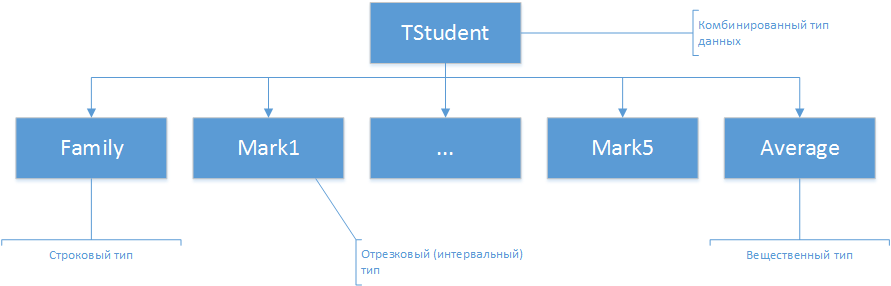
\includegraphics[scale=0.4]{images/record-01.png}
\end{figure}
\end{frame}

\subsection{Селектор записи}
\begin{frame}[fragile]
Для доступа к значению компоненты записи используется селектор записи.
\begin{block}{Селектор записи}
задается именем переменной типа запись и именем компоненты записи, разделенными точкой.	
\end{block}
\begin{alltt}
1 Ivanov.Family := 'Иванов';
2 Ivanov.Mark1 := 3;
3 Ivanov.Average := (Ivanov.Mark1 + Ivanov.Mark2 
    + Ivanov.Mark3 + Ivanov.Mark4 + Ivanov.Mark5)/5;
4 Group748[1].Mark1 := Group748[2].Mark2;
5 Group748[k] := Group748[k+1];
\end{alltt}
\end{frame} 

\begin{frame}[fragile]
Определение среднего балла
\begin{alltt}
1 type
2   TStudent = record
3      Family: string; 							{фамилия студента}
4      Mark1, Mark2, Mark3, Mark4, Mark5:2..5; 	{оценки}
5      Average: real; 							{средний балл}
6   end;
7   var
8     Group748: array[1..11] of TStudent; 
9     i: integer; 
10    TotalAverage: real;
11  begin
12    for i := 1 to 11 do
13      readln(Group748[i].Family, Group748[i].Mark1, 
           Group748[i].Mark2, Group748[i].Mark3, 
           Group748[i].Mark4, Group748[i].Mark5);
\end{alltt}
\end{frame}

\begin{frame}[fragile]
Определение среднего балла (продолжение)
\begin{alltt}
\{вычисляем средний балл каждого студента\}
14   for i := 1 to 11 do 
15     Group748[i].Average := (Group748[i].Mark1 
           + Group748[i].Mark2 + Group748[i].Mark3 
           + Group748[i].Mark4 + Group748[i].Mark5) / 5;
16   TotalAverage := 0; 
17   for i := 1 to 11 do {вычисляем средний балл группы}
18     TotalAverage := TotalAverage + Group748[i].Average;
19   TotalAverage := TotalAverage / 11; 
20   writeln('Total average:', TotalAverage:10:4);
21 end.
\end{alltt}
\end{frame}

\begin{frame}[fragile]
Сортировка выбором максимального элемента
\begin{alltt}
0 const M = 11;
1 var
2	tmp: TStudent;
3	i, j, k: integer;
4   ...	
5 begin
6   ...	
7   for i := 1 to M-1 do 
8   begin
9     k := i;
10    for j := i+1 to M do  
11      if Group748[j].Average > Group748[k].Average then 
12         k := j;  
13    tmp := Group748[k];
14    Group748[k] := Group748[i];
15    Group748[i] := tmp;
16  end;
17 end.
\end{alltt}
\end{frame}

\subsection{Оператор присоединения}
\begin{frame}[fragile]
\begin{block}{Оператор присоединения}
позволяет осуществить доступ к компонентами записи таким образом, как если бы они были простыми переменными.	
\end{block}
\begin{alltt}
1 with <Выражение> do
2   <Оператор>
\end{alltt}
\begin{itemize}
\item Выражение - выражение, имеющее значение комбинированного типа;
\item Оператор - оператор языка Pascal.
\end{itemize}
\begin{alltt}
14 for i := 1 to 11 do
15   with Group748[i] do
16     Average := (Mark1 + Mark2 + Mark3 + Mark4 + Mark5)/5;
\end{alltt}
\end{frame} 

\subsection{Вложенные записи}
\begin{frame}[fragile]
Допускается использование записи в качестве элемента другой записи.
\begin{figure}
\centering
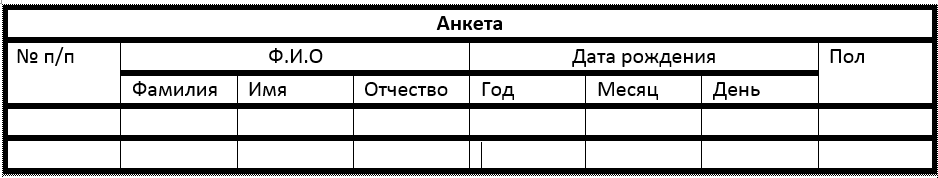
\includegraphics[scale=0.4]{images/record-02.png}
\end{figure}
\begin{alltt}
1 Type
2  TGender = (Male, Female);
3  TDate = record 
4    Day: 1..31;
5    Month: 1..12;
6    Year: 1900..2100;
7  end;  
8  TFormular = record
9    Names: record FName, SName, LName: string; end;
10   Birthday: TDate;
11   Gender: TGender;
12 end;
\end{alltt}
\end{frame} 

\begin{frame}[fragile]
\begin{alltt}
1 var
2  A: TFormular; 
3 begin
4   A.Gender := Male; \{селектор записи\}
5   A.Birthday.Year := 1991; \{селектор вложенной записи\}
6   A.Names.FName := 'Иван'; 
7   with A do \{оператор присоединения\}
8     Names.LName := 'Иванов';
9   with A.Date do \{оператор присоединения вложенной записи \}
10  begin
11    Month := 12;   
12    Day := 1;
13  end;
14 end.
\end{alltt}
\end{frame} 

\end{document}
